\documentclass[12pt]{article}
\usepackage[T1]{fontenc}
\usepackage[polish]{babel}
\usepackage[utf8]{inputenc}
\usepackage{graphicx}
\usepackage{amsmath}

\graphicspath{ {./images} }

\begin{document}

\title{{\Large}Zadanie numeryczne 10}
\date{}
\author{Jakub Heczko}

\maketitle
\section{Uwagi:}
Często będę używał sformułowania przedział naprzemiennie z punktami, chodzi mi poprsotu o tę strefę pomiedzy, w ogólności zawsze podczas tych warunków stopu chodzi o to, żeby sprawdzić jak bardzo x nam się zmienia, jeśli bedzie to nieznacząca(zalezy dla nas co to znaczy nieznaczaco, musimy okreslic blad) zmiana to przerywamy. Przedzial jest wiec dla mnie tymi dwoma punktami miedzy ktorymi szukami miejsca zerowego. W niektórych metodach, również będę sprawdzał, czy mój nowy iterat nie przyjął już od razu wartości 0(szczęśliwy traf), więc to też jest uwzględnione, ale nie we wszystkich metodach.

\section{Wprowadzenie do problemu: }
Problemem zadania było rozwiązanie równiania charakterystycznego pewnej macierzy. Zadanie sprowadzało, się do znalezienia miejsc zerowych naszej funkcji
\section{Algorytmy i rozwiązanie: }
Zacznijmy może od tego jak wygląda nasza macierz:
\[
\begin{bmatrix}
    4 & -1 & 0 \\
    -1 & 4 & -1 \\ 
    0 & -1 & 4 \\
\end{bmatrix}
\]
Nastepnie po zapisaniu i uproszczeniu wyznacznika dostajemy funkcję następującej postaci:
\begin{center}
    \begin{math}
        f(x) = -x^{3}+12x^{2}-46x+56
    \end{math}
\end{center}
Taka funkcja wygląda następująco na wykresie:
\newline
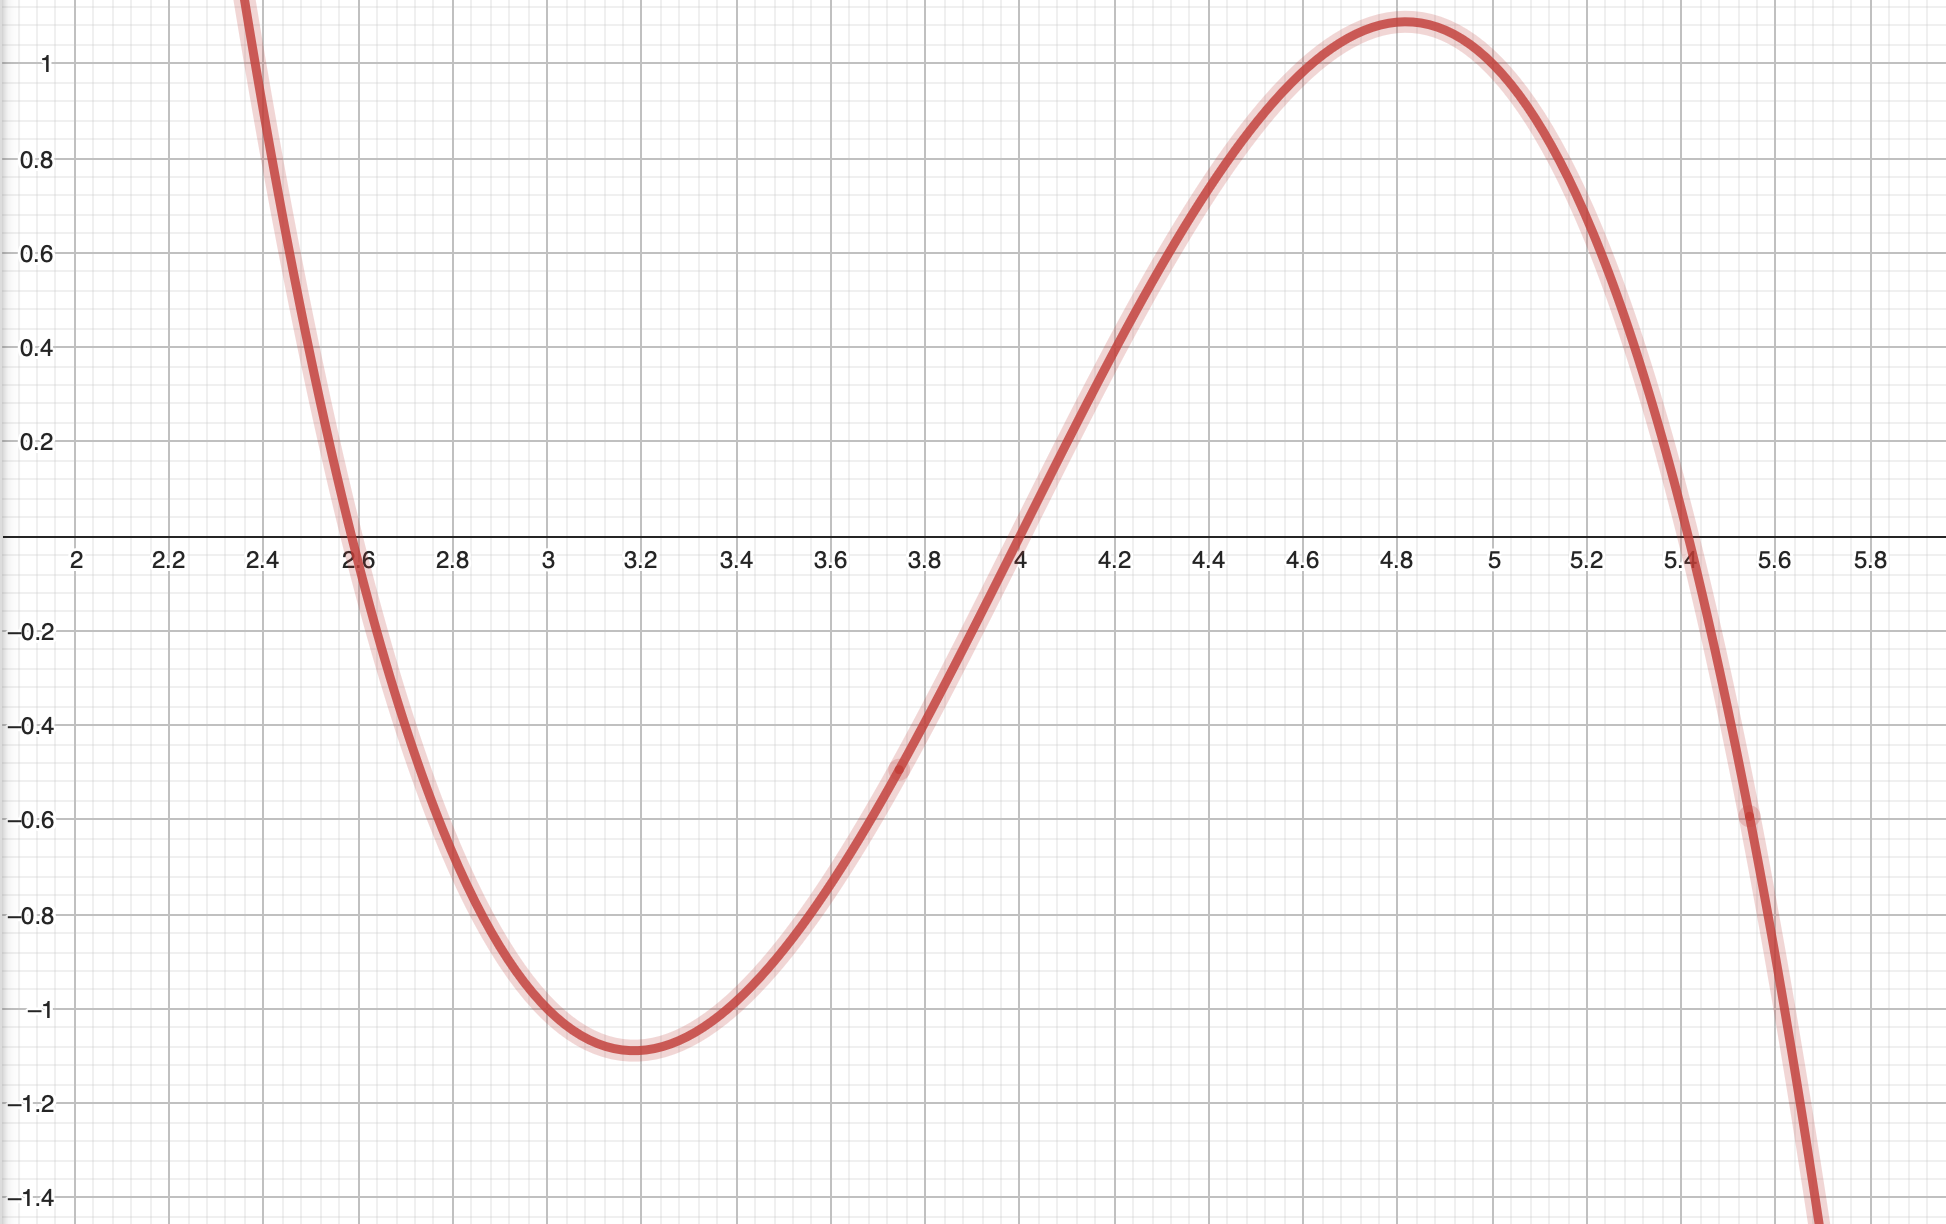
\includegraphics[width=12cm,height=8cm, keepaspectratio]{wykres_funkcja.png}
\newline
Jak widzimy osiąga ona miejsca zerowe w $x_{1} = -2,585786437626905$ oraz $x_{2} = 4$ oraz $x_{3} = 5,414213562373095$
\newline
Teraz, aby znaleźć nasze miejsca zerowe, użyje trzech funkcji, które każde z nich po kolei omówie, pierwszą będzie metodą bisekcji, nastepną metoda regula falsi i na samym końcu metoda siecznych. 
\subsection{Metoda Bisekcji:}
Metoda bisekcji jest najprostsza, z 3 wszystkich metod, działa ona następująco, musimy najpierw znaleźć dwa punkty, w których ich wartość, będą miały przeciwne do siebie znaki. Czyli można zapisać warunki początkowe, że:
\begin{center}
    \begin{math}
        f(x_{1})f(x_{2}) < 0
    \end{math}
\end{center}
Do tego należy pamiętać, że jeżeli funkcja, którego miejsca zerowego szukamy, ma miejsce zerowe o krotności parzystej, to metoda bisekcji nie zadziała, bo w okolicach miejsca zerowego znak nie będzie się zmieniał, więc nasze warunki początkowe nie działają. Ale jeżeli spełniliśmy wszystkie wymaganie to możemy zapisać, że nasza nowa współrzedna, będzie równa połowie odległości, miedzy $x_{2}$ oraz $x_{1}$, można więc zapisać, że:
\begin{center}
    \begin{math}
        x_{3} = \frac{x_{1}+x_{2}}{2}
    \end{math}
\end{center}
Teraz, należy wybrać przedział tak, aby z jednej strony był argument o ujemnej wartośći, a  z drugiej argument o wartości dodatnej, należy pamietać, że w tym przedziale musi być $x_{3}$, czyli jeżeli na początku $f(x_{1})>0$ i $f(x_{2})<0$, to jeżeli dostaniemy nasz trzeci argument, którego wartość  będzię mniejsza od zera to nasz nowy przedział będzie wyglądać następująco:
\begin{center}
    \begin{math}
        newArr = [x_{1},x_{3}]
    \end{math}
\end{center}
Analogicznie dla odwrotnej sytuacji, gdy wartość otrzymanego przybliżenia, będzię większa otrzymamy:
\begin{center}
    \begin{math}
        newArr = [x_{3},x_{2}]
    \end{math}
\end{center}
Nie musimy tutaj się martwić kolejnością, punktów, bo we wzorze na kolejne iteraty mamy dodawanie, więc poprostu dbamy o to, aby jedna wartośc była dodatnia, a druga ujemna.
\subsubsection*{Warunek stopu: }
Aby stwierdzić, czy jesteśmy wystarczająco blisko miejsca, zerowego, nie należy sprawdzać wartości jak bardzo różnią się od zera, lecz bardziej jak duży krok robimy w każdej iteracji, czyli, sprawdzamy, jak bardzo nasze przybliżenia, różnia się od siebie, czyli możemy zapisać Warunek:
\begin{center}
    \begin{math}
        |x_{n}-x_{n-1}|<\epsilon
    \end{math}
\end{center}
Ale, ponieważ w moim programie, zmienna $x_{n-1}$ znajduje się zawsze w zmiennej $x_{2}$, a $x_{3}=x_{n}$ to można, zapisać, że:
\begin{center}
    \begin{math}
        |x_{3}-x_{2}|<\epsilon
    \end{math}
\end{center}
\subsubsection*{Graficzny przykład: }
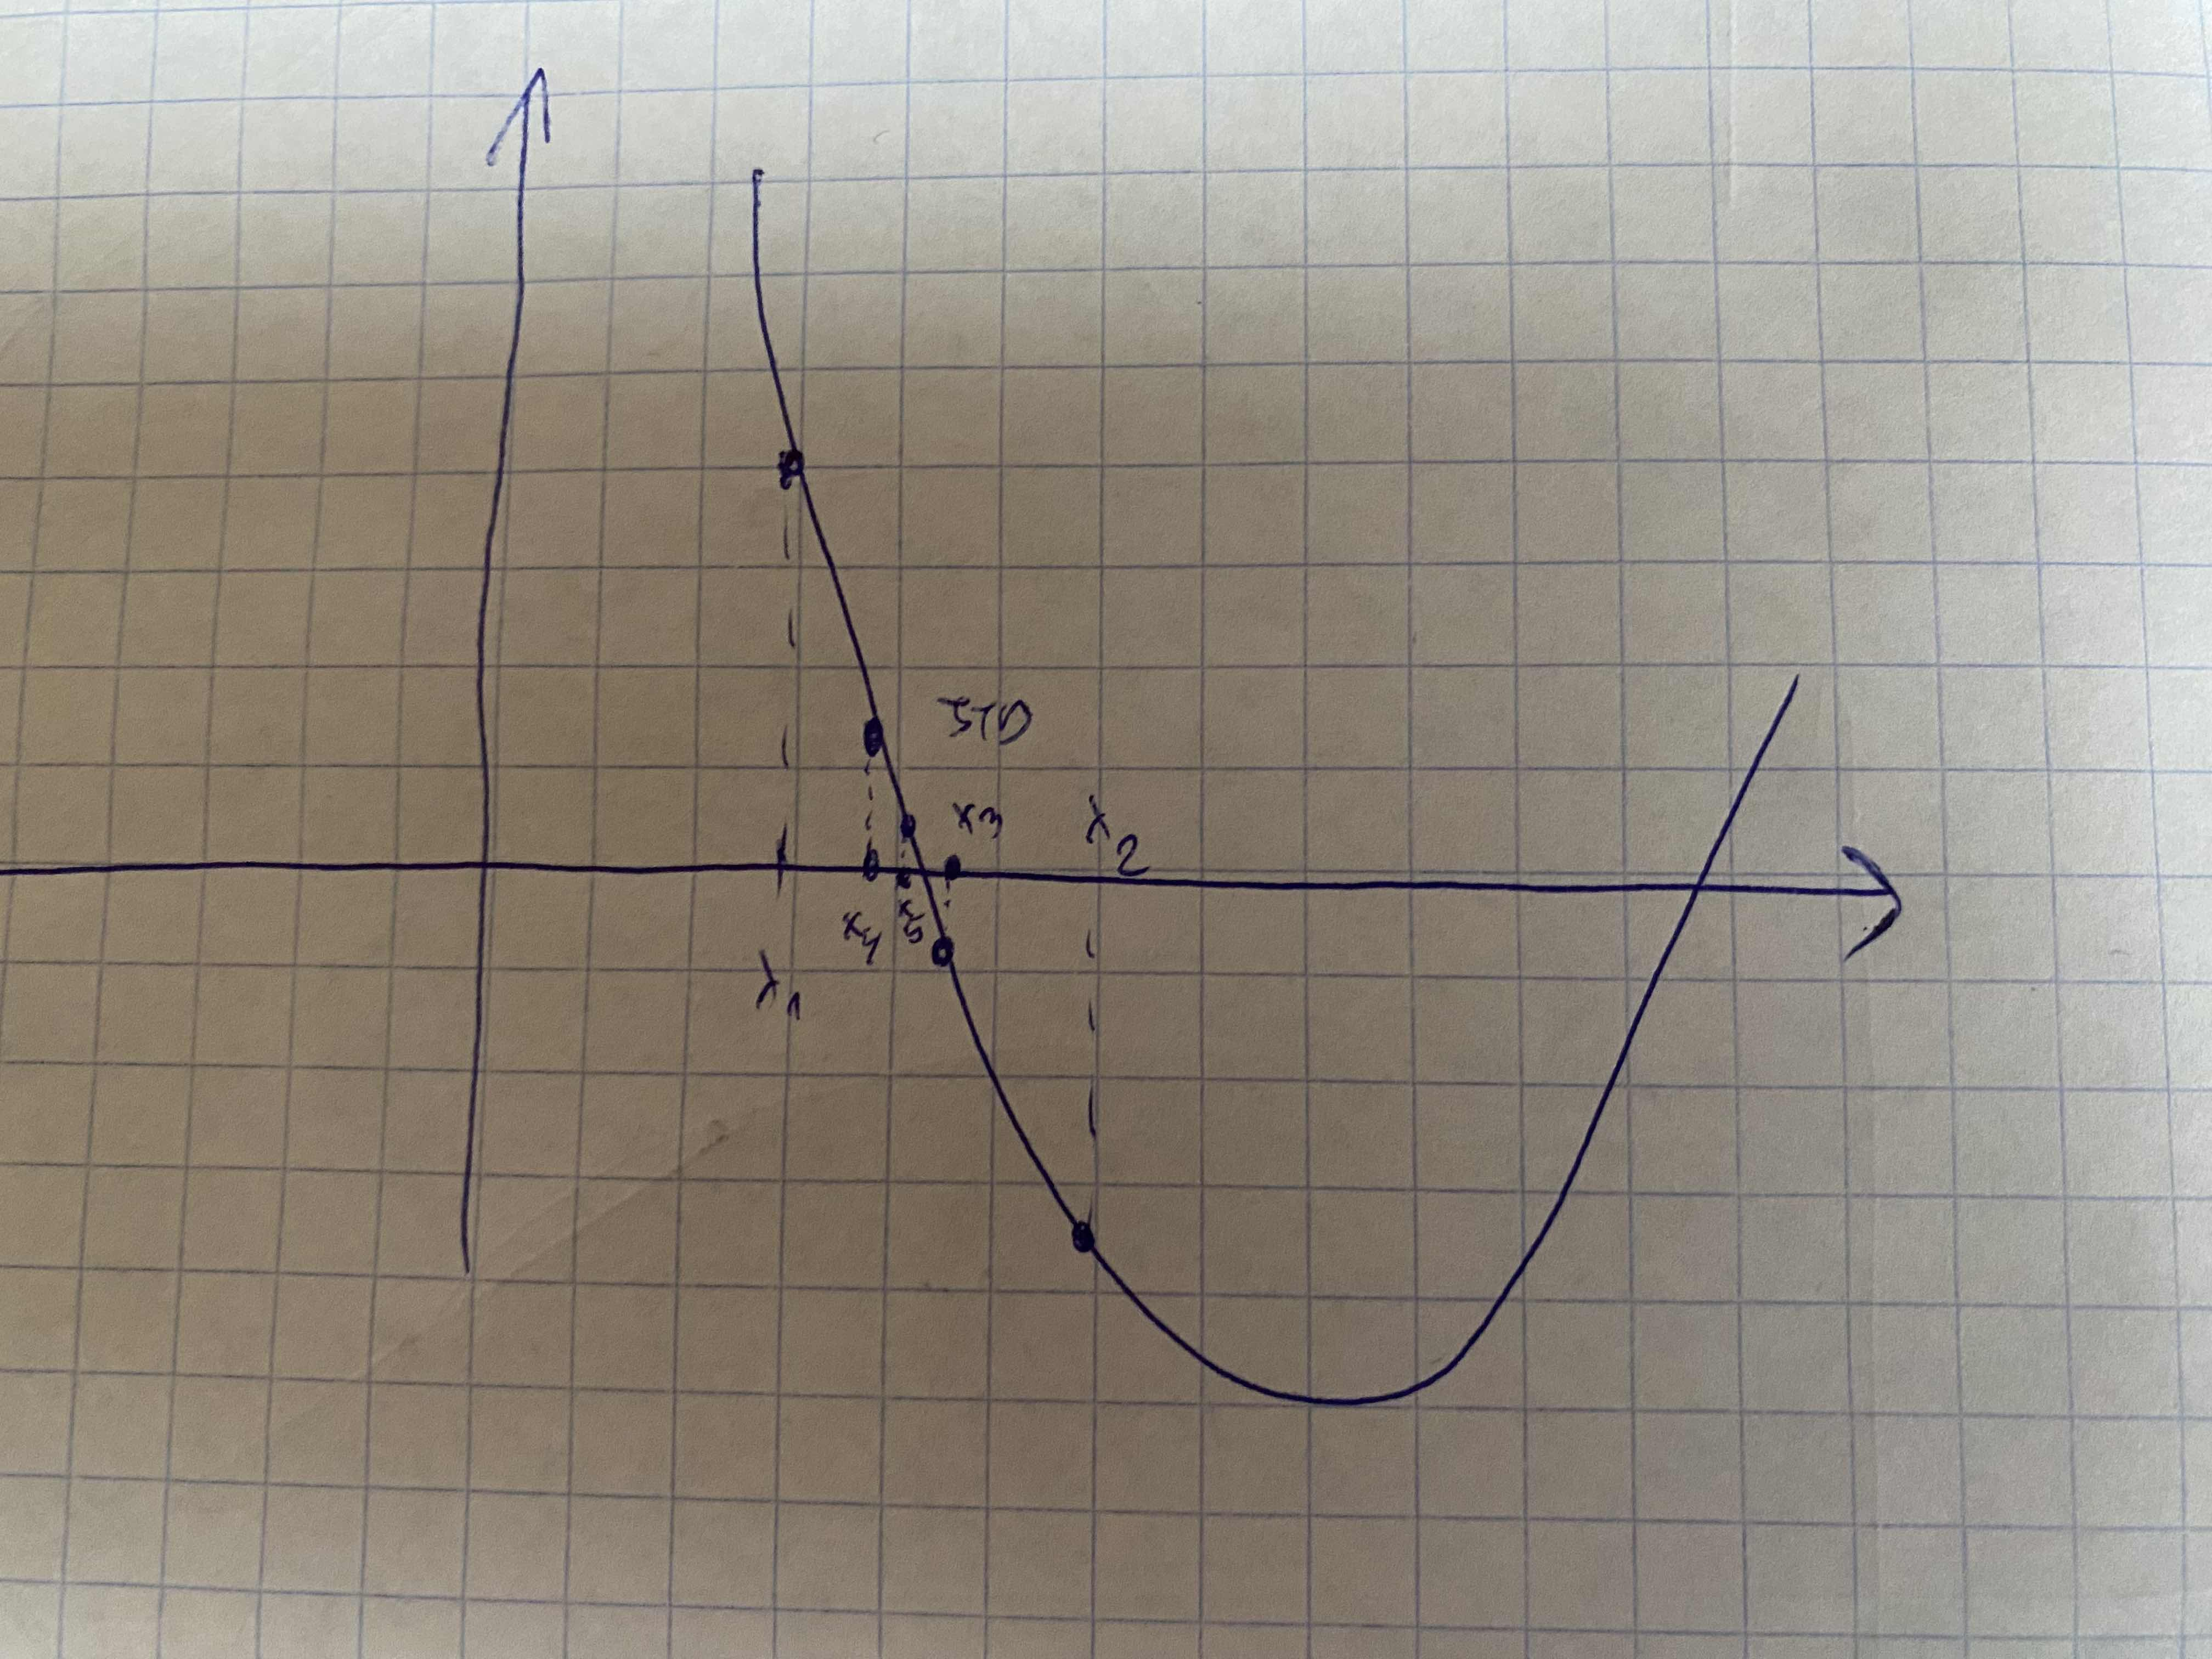
\includegraphics[width=17cm,height=8cm, keepaspectratio]{bisekcja.jpg}
\subsection{Metoda Regula Falsi:}
Reguła falsi, jest metodą, bardzo podobną do metody siecznych, czyli konstruujemy sieczną, przez dwa punkty i punkt przecięcia tej siecznej z naszą osią OX, to będzie punkt naszego nowego przybliżenia. Warunki początkowe, podobne jak w bisekcji, czyli musimy mieć dwa punkty o wartościach, które mają przeciwne znaki, i przez nie robimy sieczną(przez te punkty oczywiście), potem dostajemy punkt przybliżenia z punktu przecięcia się z osią OX, tej siecznej i to jest nasze nowe $x_{3}$, nastepnie sprawdzamy znak i na tej podstawie, robimy przedział do nastenych iteracji. Również miejsce zerowe musi być nieparzystej krotności, abyśmy mogli mieć, różne znaki po dwóch stronach miejsca zerowego. To teraz zapiszmy wzór na kolejne iteraty, czyli punkt przeciecia siecznej z osią OX:
\begin{center}
    \begin{math}
        x_{3} = \frac{f(x1)x2 - f(x2)x1}{f(x1) - f(x2)}
    \end{math}
\end{center}
Nastepnie konstrujemy przedział za pomocą następujących warunków, tutaj już musimy pamiętać, aby $x_{1}<x_{2}$ więc możemy zapisać nasze warunki na przedział, analogicznie jak w bisekcji, ale z uwzględnieniem tego co napisałem:
\begin{center}
    Jeśli $f(x_{3})f(x_{2})<=0$ to: \newline
    \begin{math}
        x1 = x3\newline
        x2 = x2
    \end{math}
\end{center}
\begin{center}
    Jeśli $f(x_{3})f(x_{1})<=0$ to: \newline
    \begin{math}
        x1 = x1\newline
        x2 = x3
    \end{math}
\end{center}
\subsubsection*{Warunek stopu:}
Tutaj na rysunku, który jest dalej pokazałem pewną własność tej metody, czasasami, może być tak, że jeden z punktów, będzie nieruchomy i sieczne, będą padać na jednej stronie, więc granica naszego przedziału, będzie zmieniać się tylko z jednej strony. Warunek jednak wszystko, będzie wyglądał tak samo, czyli sprawdzamy jak bardzo zmienia się nasz poprzedni iterat z następnym iteratem, warunek stopu wygląda następująco:
\begin{center}
    \begin{math}
        |x_{3}-x_{3_{poprzednie}}|<\epsilon
    \end{math}
\end{center}
Nie wiem czy to dobra praktyka, ale jako zakomentowany kod, zostawiłem sprawdzanie za każdym razem jak zmieniają się nasze krańce przedziałów, a nie tylko następne iteraty, kod działa tak samo. Ale jakby ten pierwszy warunek był zły, to poprostu mam następny, który bierze pod uwage dwa punkty(krańce tego przedziału, który zawężamy) wraz z jego poprzednimi krańcami
\subsubsection*{Graficzny przykład: }
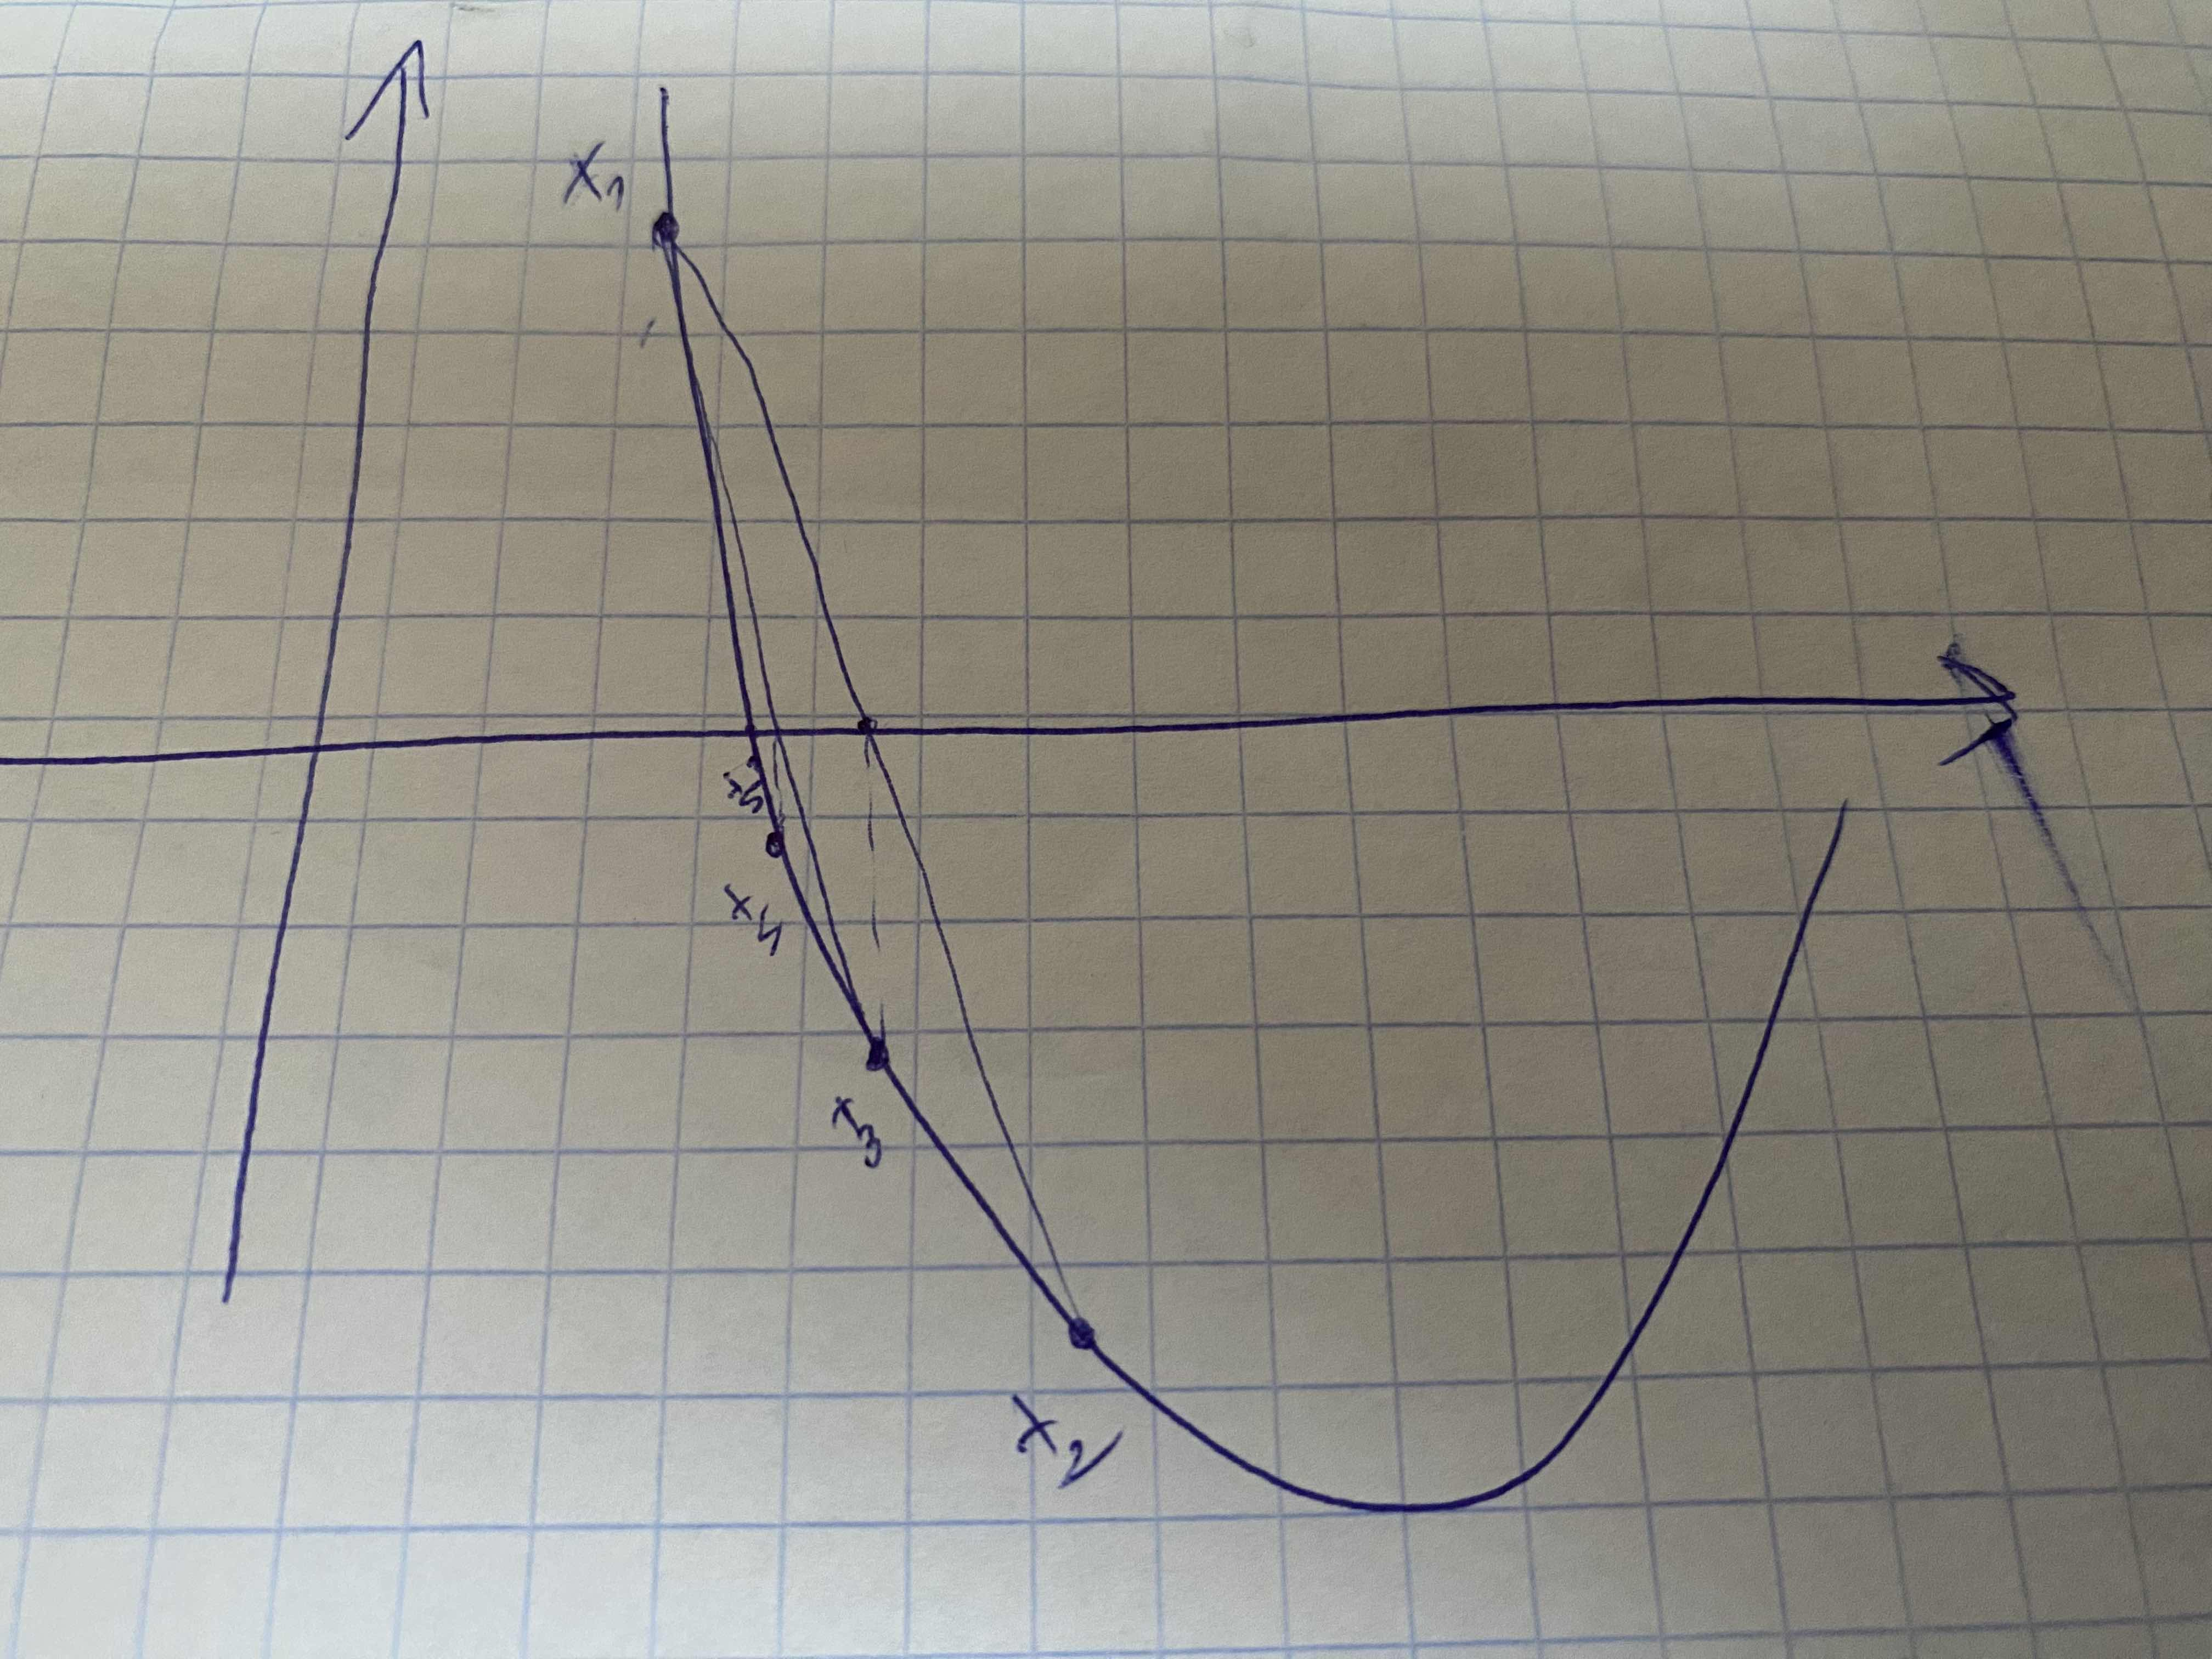
\includegraphics[width=17cm,height=8cm, keepaspectratio]{falsi.jpg}
\newline
A tutaj obserwacja o nieruchomym punkcie: \newline
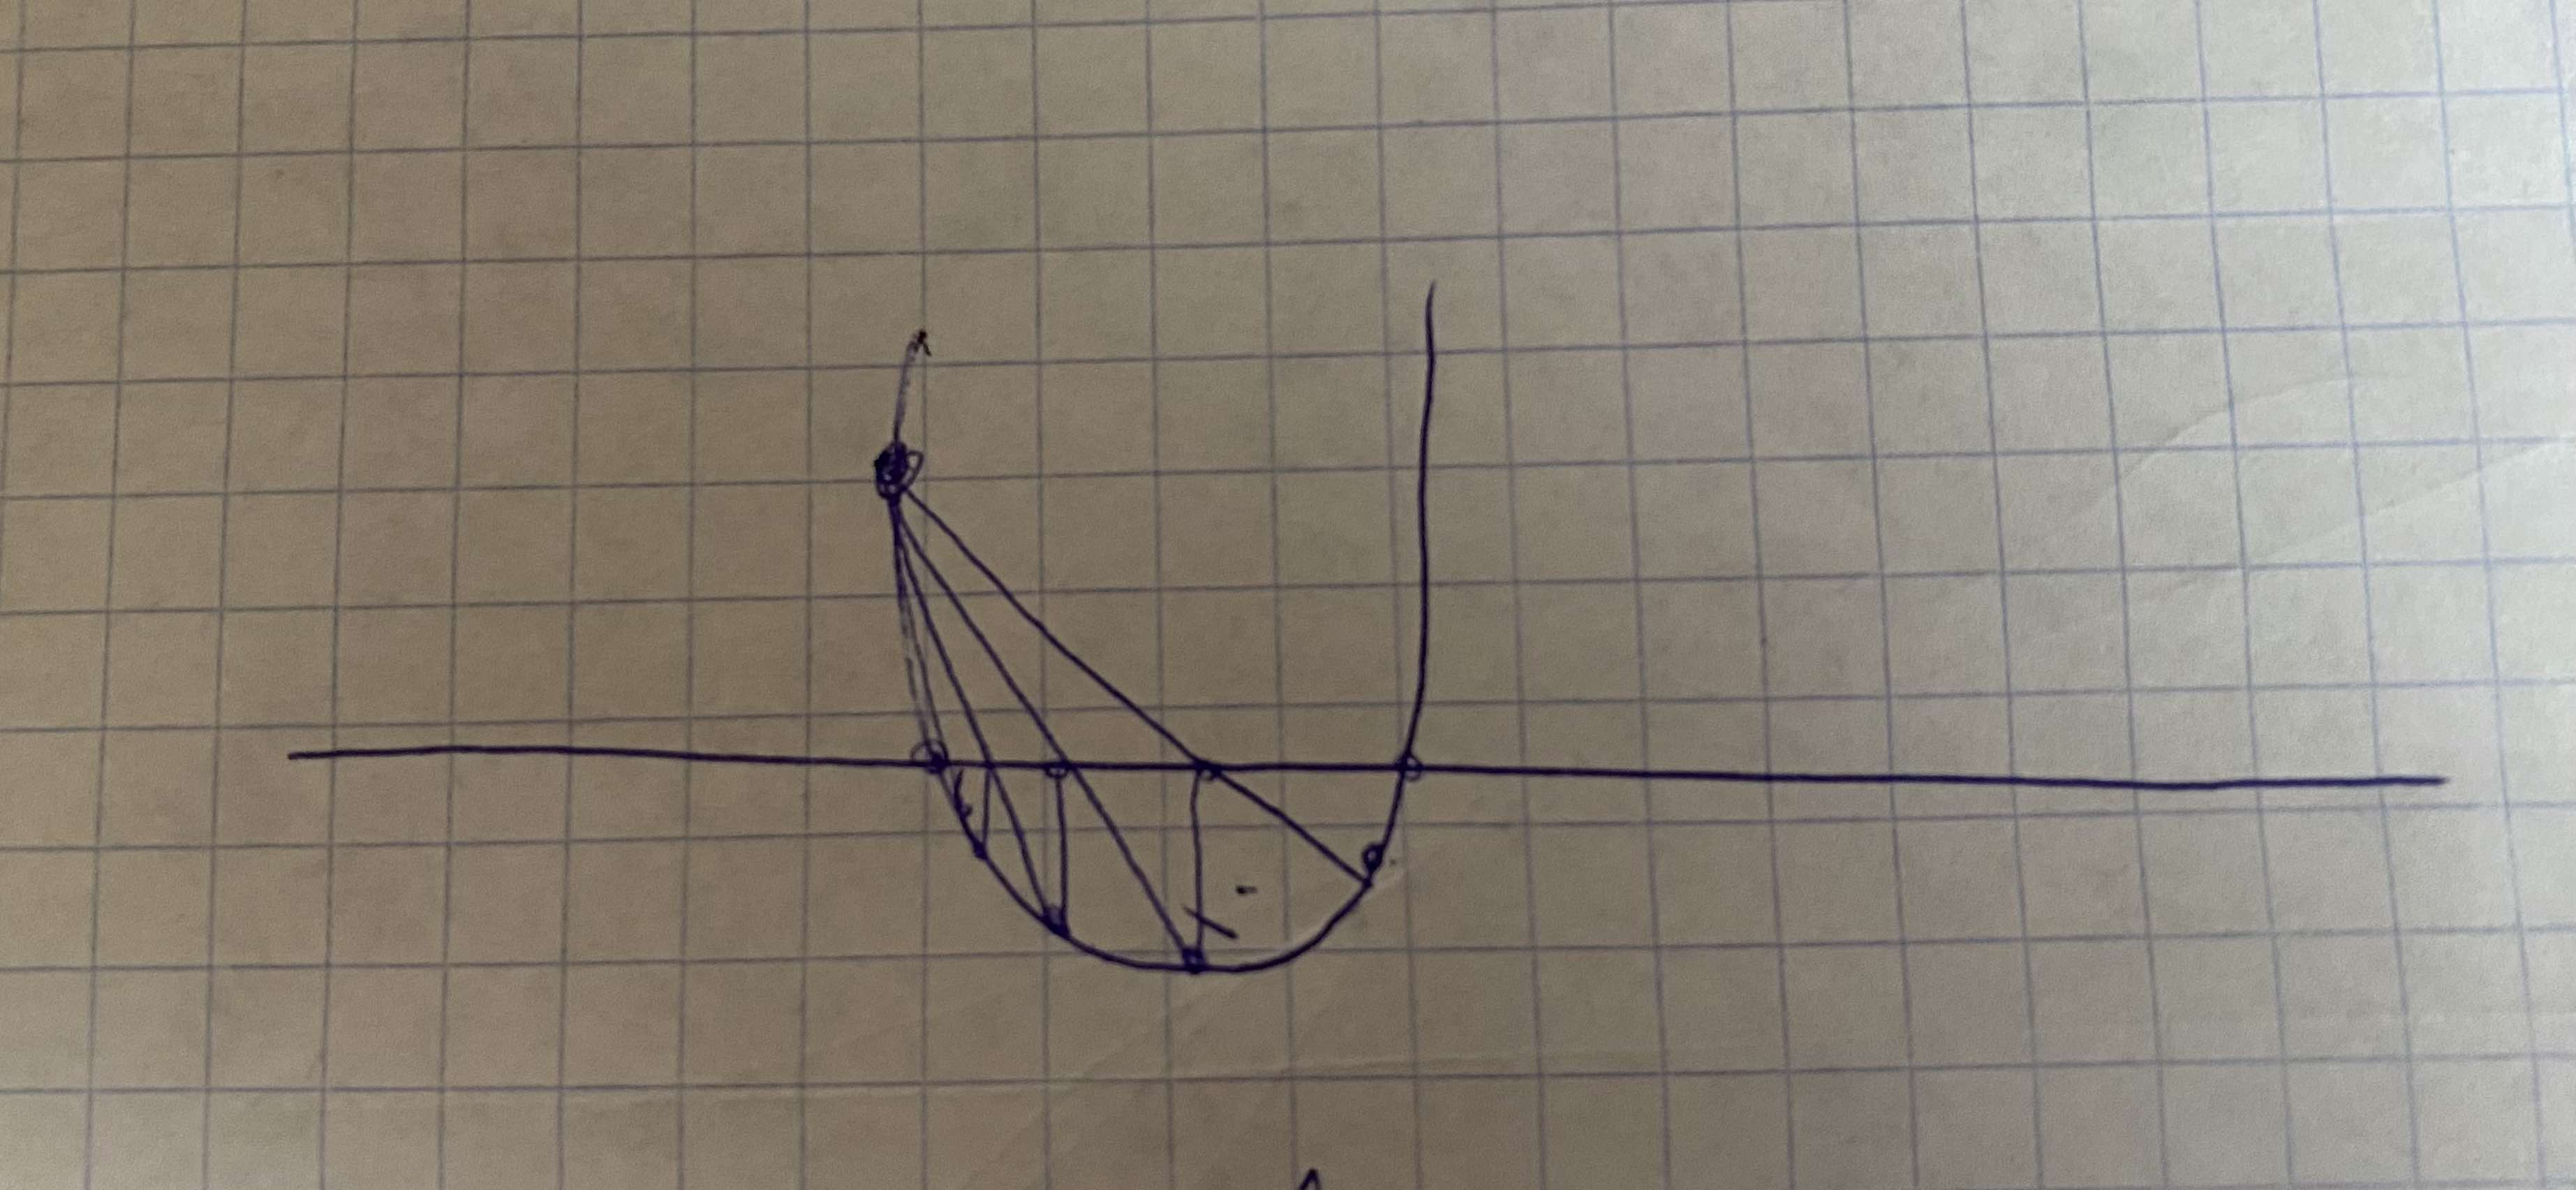
\includegraphics[width=17cm,height=8cm, keepaspectratio]{falsi_obserwacja.jpg}
\subsection{Metoda Siecznych:}
Metoda ta jest naprawde podobna do regula falsi, ale z kilkama znacznymi zmianami, po pierwsze dobór punktów startowych, nie ma znaczenia jaki bedzie znak tych punktów, bierzemy dwa dowolne, również krotność miejsca zerowego nie ma znaczenia, bo nie patrzymy na znak w kolejnych iteracjach, również jak w regula falsi, robimy sieczną przez dwa punktu $x_{1}$ oraz $x_{2}$ potem punkt przecięcia z osią OX zapisujemy w $x_{3}$. Istotnie również metoda ta nie ma zagwarantowanej zbieżności o czym wspomnę później. Następnie kolejna para punktów zawsze będzie wyglądała następująco:
\begin{center}
    \begin{math}
        [x_{2},x_{3}]
    \end{math}
\end{center}
Oczywiście punkt $x_{3}$ liczymy tak jak w regula falsi czyli konstruując sieczną przez dwa punkty:
\begin{center}
    \begin{math}
        x_{3} = \frac{f(x1)x2 - f(x2)x1}{f(x1) - f(x2)}
    \end{math}
\end{center}
\subsubsection*{Warunek Stopu: }
Warunek stopu będzie wyglądał następująco, czyli patrzymy na to jak zmienia się nasz iterat z każdą iteracja, czyli możemy zapisać, że:
\begin{center}
    \begin{math}
        |x_{3}-x_{2}|<\epsilon
    \end{math}
\end{center}
Trzeba pamiętać, że nasze stare $x_{3}$ bedzie zapisane w zmiennej $x_{2}$ dlatego, możemy sobie tak ułatwić sprawę. Tak jak wspomniałem, metoda ta niekoniecznie, może być zbieżna, dlatego trzeba ustalić jakąś maksymalną liczbę iteracji, po której stwierdzimy, że nie udało nam się znaleźc miejsca zerowego
\subsubsection*{Graficzny przykład: }
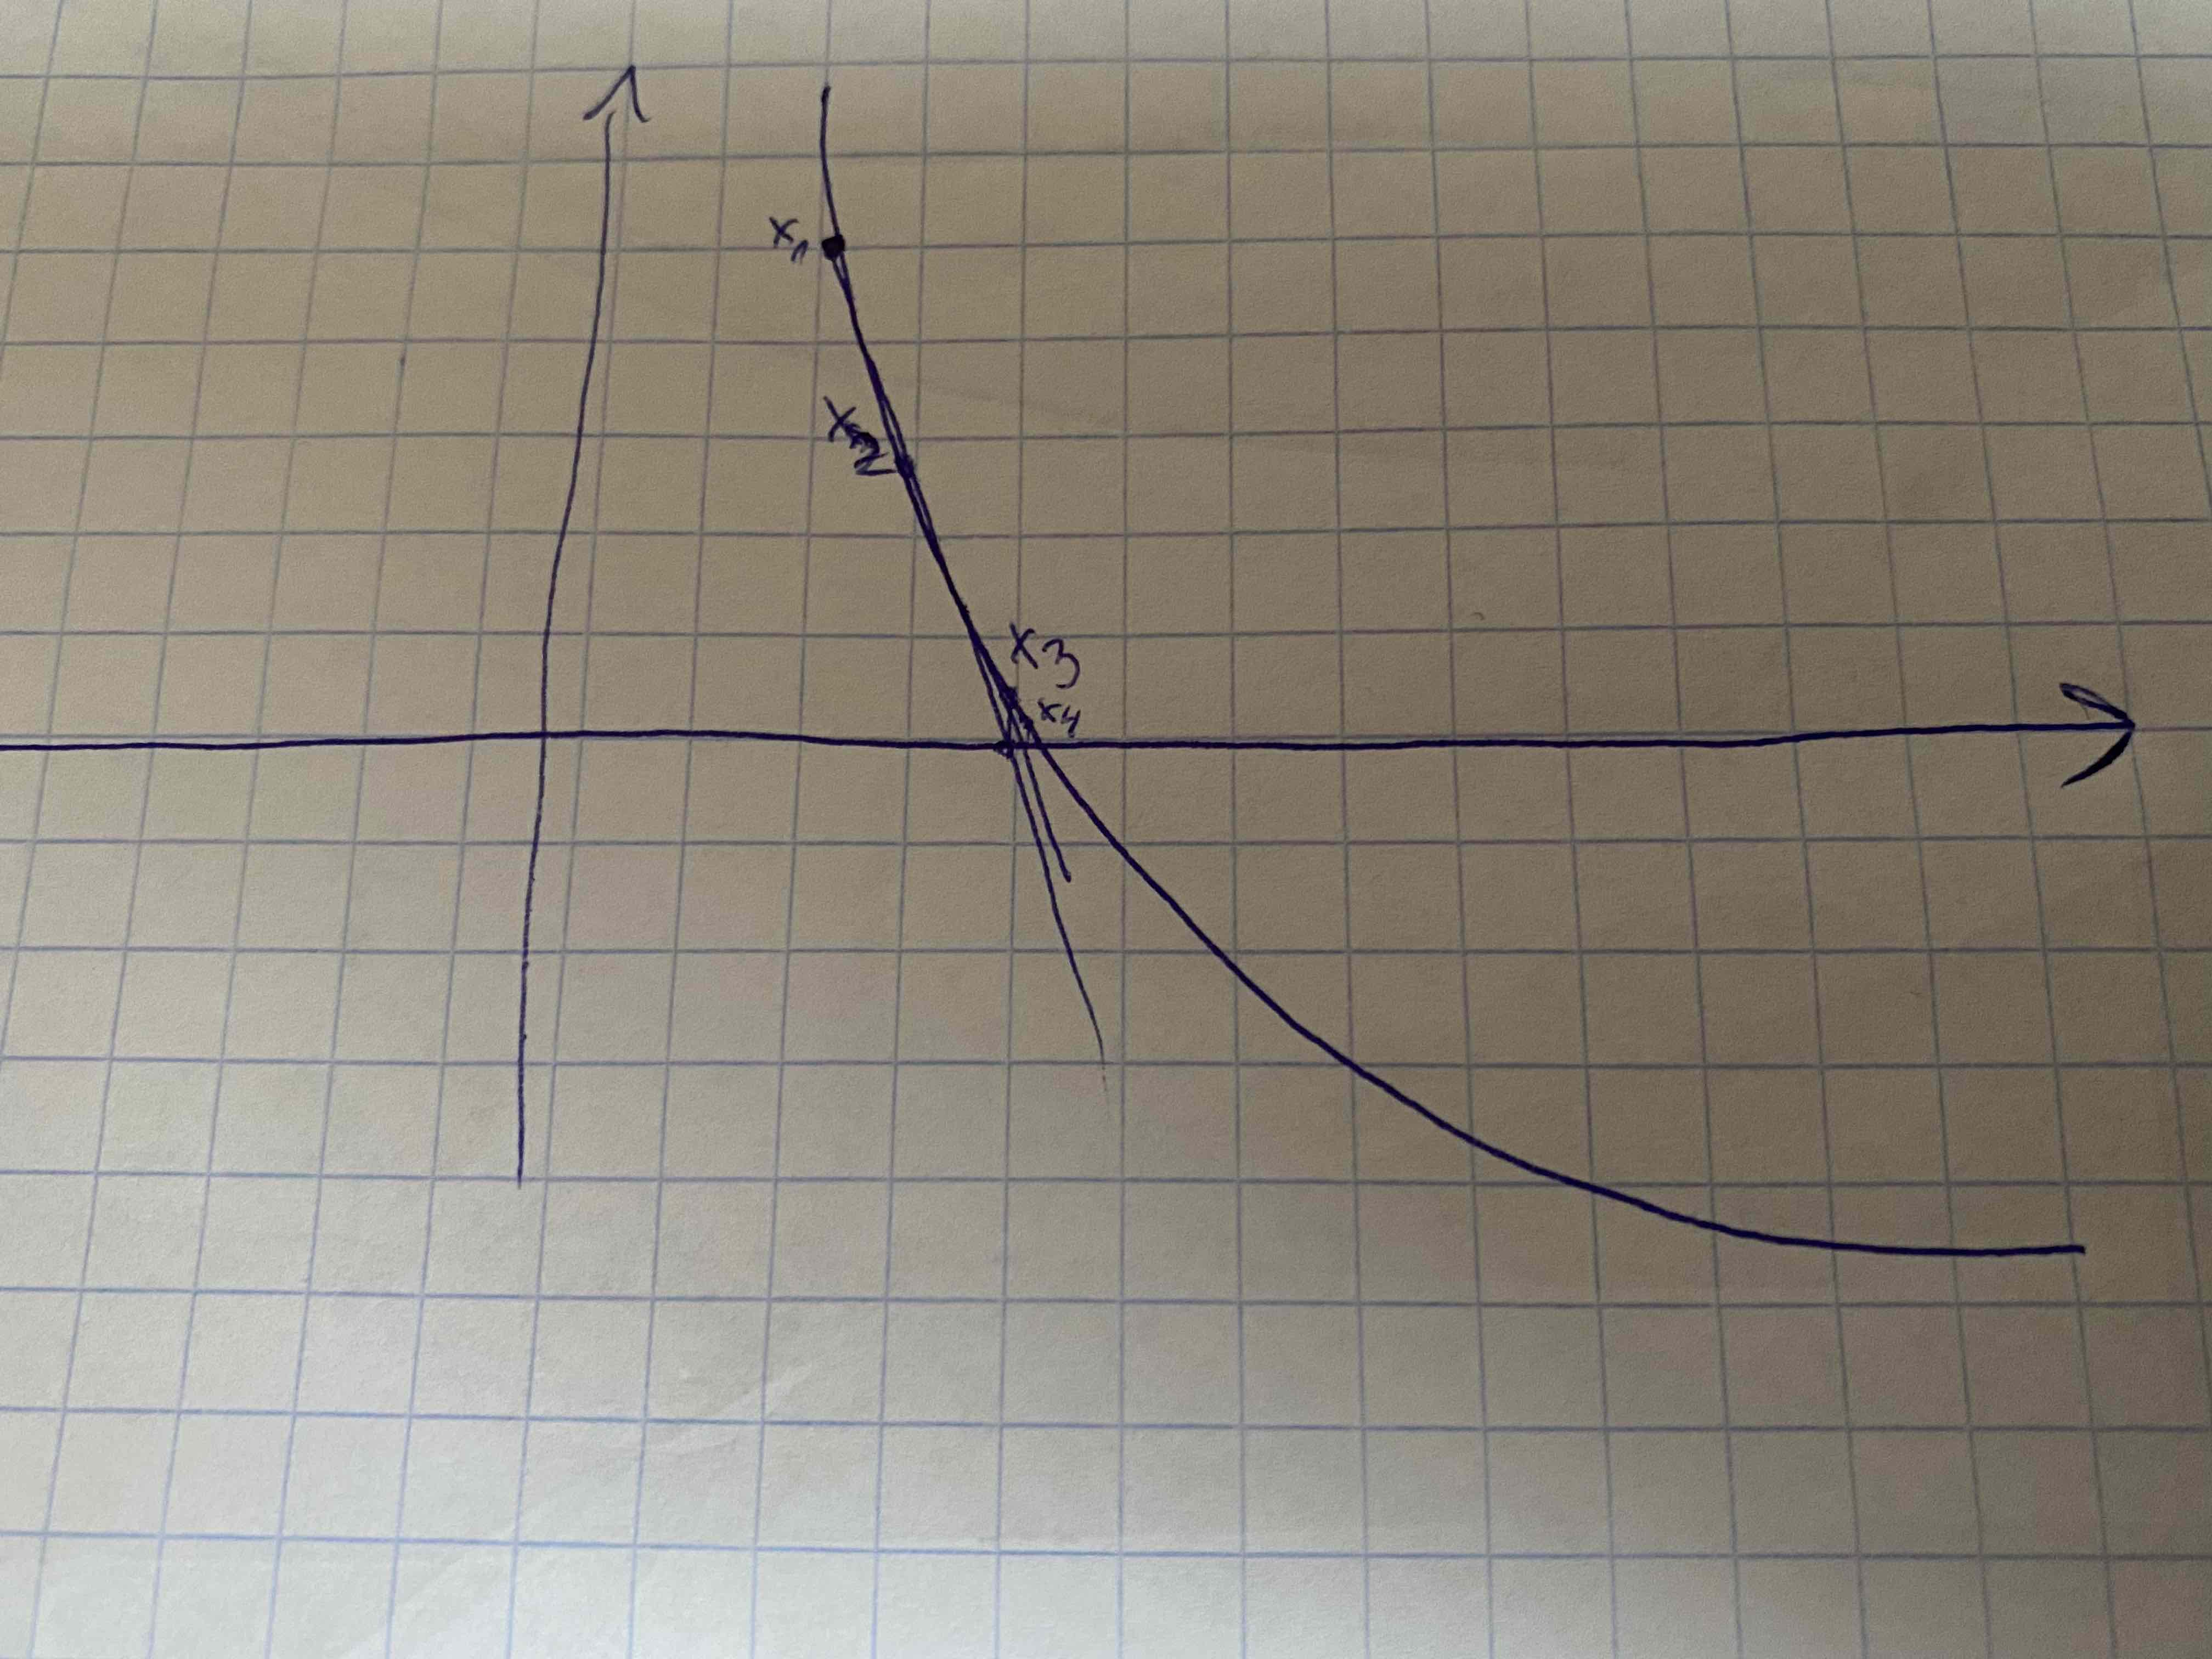
\includegraphics[width=17cm,height=8cm, keepaspectratio]{sieczne.jpg}
\section{Wyniki:}
Bisekcja iteracje:  79\newline
Bisekcja: [2.5857864394783974, 4.000000007450581, 5.414213560521603]\newline
Falsi iteracje:  40\newline
Falsi:  [2.5857864434036886, 4.0, 5.414213556596305]\newline
Sieczne iteracje:  15\newline
Siecznych:  [2.5857864376268997, 4.0, 5.414213562373092]\newline
Jak widać najszybciej z nich wszystkich poradziła sobie metoda siecznych, która praktycznie trzy-krotnie skróciła naszą ilośc iteracji. Jest ona zdecydowanie najsyzbsze z tych 3 omówionych
\end{document}